\section{Pointers: Important Concepts}
\label{sec:Pointers-ImportantConcepts}
%~\cref{sec:Pointers-ImportantConcepts}
\subsection{Passing Arguments with Pointers}
\label{subsec:Pointers-02-ImportantConcepts-PassingArguments}
%~\cref{subsec:Pointers-02-ImportantConcepts-PassingArguments}

There are three forms of passing arguments to a function. One of them is possible through the use of pointers.
\begin{itemize}
    \item Passing by value
    \item Passing by reference with a reference argument\\
    \begin{minipage}{\MPWxXXSxLISTING\textwidth} % = 0.36 times \textwidth
    \vspaceTextToListing % =\vspace{0.1cm}
    \begin{CPPCode}
int x{2};
SquareByReference(x)
cout ¿<¿¿<¿ "x is" ¿<¿¿<¿ x 
    \end{CPPCode}
    \begin{Terminal}
Output:
x is 4
    \end{Terminal}
    \end{minipage}
    \hspaceListingXSToListingXS
    \begin{minipage}{\MPWxXSxLISTING\textwidth} % = 0.36 times \textwidth
    \vspaceTextToListing % =\vspace{0.1cm}
    \begin{CPPCode}
squareByReference(int&) // Prototype

squareByReference(int& numberRef)
{
    numberRef *= numberRef;
}
    \end{CPPCode}
    \end{minipage}
    
    \item Passing by reference with a pointer argument\\
    \begin{minipage}{\MPWxXXSxLISTING\textwidth} % = 0.36 times \textwidth
    \vspaceTextToListing % =\vspace{0.1cm}
    \begin{CPPCode}
int x{2};
SquareByPtrRef(&x)
cout ¿<¿¿<¿ "x is" ¿<¿¿<¿ x 
    \end{CPPCode}
    \begin{Terminal}
Output:
x is 4
    \end{Terminal}
    \end{minipage}
    \hspaceListingXSToListingXS
    \begin{minipage}{\MPWxXSxLISTING\textwidth} % = 0.36 times \textwidth
    \vspaceTextToListing % =\vspace{0.1cm}
    \begin{CPPCode}
squareByPtrRef(int*)// Prototype

squareByPtrRef(int* nPtr)
{
    *nPtr = *nPtr * *nPtr
}
    \end{CPPCode}
    \end{minipage}
\end{itemize}

\noindent Passing a \textbf{variable} by reference with a pointer \textbf{does not actually pass anything by reference} a pointer to that variable is passed by value and is copied into the function’s corresponding pointer parameter. The called function can then access that variable in the caller simply by \textbf{dereferencing} the pointer, thus accomplishing pass-by-reference.\\

\noindent \textbf{Remark}. When a pointer to an object is passed, only a copy of the address of the object must be made, the object itself is not copied.

\subsection{\CppCommonCode{const} with Pointers}
\label{subsec:Pointers-02-ImportantConcepts-02-const-with-Pointers}
%~\cref{subsec:Pointers-02-ImportantConcepts-02-const-with-Pointers}

%% Counters
\newcounter{ctrPassPtrToFcn} % a <- ch00-Important row counter
\stepcounter{ctrPassPtrToFcn}

Keyword \CppCommonCode{const} enables you to inform the compiler that the value of a particular variable should \textbf{not} be modified. This is usefull when using built-in arrays (See Section~\cref{subsec:Built-In-Arrays}) as they are passed by reference and could easily be changed in the called funcion. An attempt to modify a const value is a compilation error.

\subsection{Passing a pointer to a function}
\label{subsec:Pointers-02-ImportantConcepts-03-Pass-Pointer-to-fcn}
%~\cref{subsec:Pointers-02-ImportantConcepts-03-Pass-Pointer-to-fcn}
There are four ways to a pass a pointer to a function:
\begin{table}[!h]
	\centering                       % Center your table
	\begin{tblr}{vspan=default,
                     colspec={Q[r,m]|Q[c,m]|Q[l,m]|Q[l,m]|},
                     column{3}={4.0cm}}     % set length 
    \SetHline{2-4}{black}
    & Way & Ptr is constant ? & Data is constant? \\
    \SetHline{2-4}{black}
    & \arabic{ctrPassPtrToFcn}                             & a \textbf{non}constant pointer & to \textbf{non}constant data \\
    \SetHline{2-4}{black}   %E
    & \stepcounter{ctrPassPtrToFcn}\arabic{ctrPassPtrToFcn} & a \textbf{non}constant pointer & to \hspace{0.65cm}constant data \\
    \SetHline{2-4}{black}
    & \stepcounter{ctrPassPtrToFcn}\arabic{ctrPassPtrToFcn} & a \hspace{0.65cm}constant pointer & to \textbf{non}constant data \\
    \SetHline{2-4}{black}
    & \stepcounter{ctrPassPtrToFcn}\arabic{ctrPassPtrToFcn} & a \hspace{0.65cm}constant pointer & to \hspace{0.65cm}constant data\\
    \SetHline{2-4}{black} 
    \end{tblr}
	\caption{Main abbreviations}
 	\label{tab:t-Pointers-Ways-Pass-PtrToFcn}
\end{table}

%%%%%%%%%%%%% SUBSUBSECTION PART 1
\subsubsection{A (\underline{non}constant) pointer to (\underline{non}constant) data}
    \begin{minipage}{\MPWxXSxLISTING\textwidth} % = 0.36 times \textwidth
    \vspaceTextToListing % =\vspace{0.1cm}
    \begin{CPPCode}
int* fooPtr
    \end{CPPCode}
    \end{minipage}\\
\begin{itemize}
    \item the data can be modified through the dereferenced pointer, and
    \item the pointer can be modified to point to other data.
\end{itemize}

%%%%%%%%%%%%% SUBSUBSECTION PART 2
\subsubsection{A (\underline{non}constant) pointer to constant data}
    \begin{minipage}{\MPWxXXXSxLISTING\textwidth} % = 0.36 times \textwidth
    \vspaceTextToListing % =\vspace{0.1cm}
    \begin{CPPCode}
const int* fooPtr   //or
int const* fooPtr
    \end{CPPCode}
    \end{minipage}
    \hspaceListingXSToListingXS
\begin{minipage}{\MPWxSxLISTING\textwidth} % = 0.36 times \textwidth
    \vspaceTextToListing % =\vspace{0.1cm}
    \begin{Terminal}
fooPtr is a (non-constant) ptr to an int. constant
fooPtr is a (non-constant) ptr to a constant int.
    \end{Terminal}
    \end{minipage}\\
    
\begin{itemize}
    \item a pointer that can be modified to point to \textbf{any} data of the appropriate type, but
    \item the data which it points \textbf{cannot} be modified through that pointer
\end{itemize}
\begin{minipage}{\MPWxXSxLISTING\textwidth} % = 0.36 times \textwidth
    \vspaceTextToListing % =\vspace{0.1cm}
    \begin{CPPCode}
int main
{
    int y{0};
    \\ ¿$\downarrow$¿ illegal mod 
    f(&y);      
}
    \end{CPPCode}
\end{minipage}
\hspaceListingXSToListingXS
\begin{minipage}{\MPWxXSxLISTING\textwidth} % = 0.36 times \textwidth
    \vspaceTextToListing % =\vspace{0.1cm}
    \begin{CPPCode}
void f(const int*); //prototype

void f(const int* xPtr)
{
    *xPtr = 100;    // error
}
    \end{CPPCode}
\end{minipage}\\

\noindent In the example we tried to modify a \CppCommonCode{const} object\\
\begin{minipage}{\MPWxSxLISTING\textwidth} % = 0.36 times \textwidth
    \vspaceTextToListing % =\vspace{0.1cm}
    \begin{Terminal}
Output:
In function "void f(const int*)":
error: assignment of read-only location "* xPtr"
    \end{Terminal}
\end{minipage}\\

%%%%%%%%%%%%% SUBSUBSECTION PART 3
\subsubsection{A constant pointer to (\underline{non}constant) data}
    \begin{minipage}{\MPWxXXXSxLISTING\textwidth} % = 0.36 times \textwidth
    \vspaceTextToListing % =\vspace{0.1cm}
    \begin{CPPCode}
int* const fooPtr
    \end{CPPCode}
    \end{minipage}
    \hspaceListingXSToListingXS
\begin{minipage}{\MPWxSMALLxLISTING\textwidth} % = 0.36 times \textwidth
    \vspaceTextToListing % =\vspace{0.1cm}
    \begin{Terminal}
fooPtr is a const. ptr who points to an (nonconst.) integer
    \end{Terminal}
    \end{minipage}\\
\begin{itemize}
    \item always points to the same memory location, and
    \item the data at that location can be modified through the pointer.
\end{itemize}
\begin{minipage}{\MPWxXSxLISTING\textwidth} % = 0.36 times \textwidth
    \vspaceTextToListing % =\vspace{0.1cm}
    \begin{CPPCode}
int main
{
    int x,y;
    int* const ptr{&x};
    
    *ptr = 7;
    ptr = &y    // error     
}
    \end{CPPCode}
\end{minipage}
\\

\noindent In the example we tried to modify a \CppCommonCode{const} ptr\\
\begin{minipage}{\MPWxSxLISTING\textwidth} % = 0.36 times \textwidth
    \vspaceTextToListing % =\vspace{0.1cm}
    \begin{Terminal}
Output:
"ptr": you cannot assign to a variable that is const
    \end{Terminal}
\end{minipage}\\


%%%%%%%%%%%%% SUBSUBSECTION PART 4
\subsubsection{A constant pointer to constant data}
\begin{minipage}{\MPWxXXXSxLISTING\textwidth} % = 0.36 times \textwidth
    \vspaceTextToListing % =\vspace{0.1cm}
    \begin{CPPCode}
const int* const fooPtr
    \end{CPPCode}
    \end{minipage}
\hspaceListingXSToListingXS
\begin{minipage}{\MPWxSxLISTING\textwidth} % = 0.36 times \textwidth
    \vspaceTextToListing % =\vspace{0.1cm}
    \begin{Terminal}
fooPtr is a constant ptr to an int. constant
    \end{Terminal}
    \end{minipage}\\
    
\begin{itemize}
    \item such a pointer always points to the same memory location, and
    \item the data at that location cannot be modified via the pointer.
\end{itemize}


\subsection{Pointers Notations and Built-in Arrays}
\label{subsec:Pointers-02-ImportantConcepts-Ptrs-and-BuiltInArrays}
%~\cref{subsec:Pointers-02-ImportantConcepts-Ptrs-and-BuiltInArrays}

We saw the definition of built-in arrays in Section~\ref{subsec:Built-In-Arrays}. Pointers allow us to do any operation involving array subscripting. As an example assume \CppVar{v}, a built-in array of int has its first element at memory location $3000$.  e.g.\\
\begin{minipage}{\MPWxXXSxLISTING\textwidth} % = 0.36 times \textwidth
    \vspaceTextToListing % =\vspace{0.1cm}
    \begin{CPPCode}
int v[5]{10,11,12,13,14};
int* vPtr{v};
    \end{CPPCode}
    \end{minipage}
\hspaceListingXSToListingXS
\begin{minipage}{\MPWxSxLISTING\textwidth} % = 0.36 times \textwidth
    \vspaceTextToListing % =\vspace{0.1cm}
    \begin{CPPCode}
//also possible as
int* vPtr{&v[0]}; // ¿$\equiv$¿ vPtr{v}
    \end{CPPCode}
    \end{minipage}\\

\noindent In the old-classic way:\\
\begin{minipage}{\MPWxXXSxLISTING\textwidth} % = 0.36 times \textwidth
    \vspaceTextToListing % =\vspace{0.1cm}
    \begin{CPPCode}
int v[5]{10,20,30,40,50};
int* vPtr;
vPtr = v;
    \end{CPPCode}
    \end{minipage}
\hspaceListingXSToListingXS
\begin{minipage}{\MPWxSxLISTING\textwidth} % = 0.36 times \textwidth
    \vspaceTextToListing % =\vspace{0.1cm}
    \begin{CPPCode}
//also possible as
int* vPtr;
int* vPtr = &v[0]; // ¿$\equiv$¿ (vPtr = v) ¿$\equiv$¿ vPtr{v}
    \end{CPPCode}
    \end{minipage}\\

\noindent To refer to an element of the built-in array, e.g. 40, it is possible as:\\
\begin{minipage}{\MPWxXXXXSxLISTING\textwidth} % = 0.36 times \textwidth
    \vspaceTextToListing % =\vspace{0.1cm}
    \begin{CPPCode}
// Option 1
v[3]
    \end{CPPCode}
    \end{minipage}
\hspaceListingXSToListingXS
\begin{minipage}{\MPWxXXXXSxLISTING\textwidth} % = 0.36 times \textwidth
    \vspaceTextToListing % =\vspace{0.1cm}
    \begin{CPPCode}
// Option 2
*(v+3)
    \end{CPPCode}
    \end{minipage}
\hspaceListingXSToListingXS
\begin{minipage}{\MPWxXXXXSxLISTING\textwidth} % = 0.36 times \textwidth
    \vspaceTextToListing % =\vspace{0.1cm}
    \begin{CPPCode}
// Option 3
*(vPtr+3)
    \end{CPPCode}
    \end{minipage}
\hspaceListingXSToListingXS
\begin{minipage}{\MPWxXXXXSxLISTING\textwidth} % = 0.36 times \textwidth
    \vspaceTextToListing % =\vspace{0.1cm}
    \begin{CPPCode}
// Option 3
vPtr[3]
    \end{CPPCode}
    \end{minipage}\\

\noindent To refer to the \textbf{address} of an element of the built-in array, it is possible as:\\
\begin{minipage}{\MPWxXXXSxLISTING\textwidth} % = 0.36 times \textwidth
    \vspaceTextToListing % =\vspace{0.1cm}
    \begin{CPPCode}
// Option 1
&v[3]
    \end{CPPCode}
    \end{minipage}
\hspaceListingXSToListingXS
\begin{minipage}{\MPWxXXXSxLISTING\textwidth} % = 0.36 times \textwidth
    \vspaceTextToListing % =\vspace{0.1cm}
    \begin{CPPCode}
// Option 2
vPtr + 3
    \end{CPPCode}
    \end{minipage}\\
%%%%%%%%%%%%%%%%%%%%%%%% END going through array
% no numbers listing
% \begin{lstlisting}[frame=tlrb,numbers=none,mathescape=true,escapechar=\%,columns=flexible]

% \begin{minipage}{.9\textwidth}
% \begin{lstlisting}[frame=tlrb,showlines=htrue,firstnumber=1,mathescape=true,escapechar=\%,columns=flexible]
% //code here
% \end{lstlisting}
% \end{minipage}

% \begin{lstlisting}[frame=tlrb,showlines=htrue,firstnumber=1,mathescape=true,escapechar=\%,columns=flexible]
% //Program 12.1
% \end{lstlisting}
    
%reference:
%~\ref{tab:t_ch11_UART_Registers} tab:t_ch12_edgeTriggeredModes
%~\ref{fig:RT_ch01} 
%\texttt{Ascii}
%\texttt{UART}
%\texttt{mailbox}
%\texttt{FIFO}
%\texttt{I/O}
%\underline{}
%$\texttt{b}_0$
%\sim = ~

%percent
%n%\%%10;

%for loops
% \newcounter{nnCount}
% \forloop{nnCount}{0}{\value{nnCount}<8}{&IME }  
% \forloop{nnCount}{0}{\value{nnCount}<8}{&PMC\arabic{nnCount} }

%Apostroph:
%\textquotesingle

%Equation array
% \begin{eqnarray*}
%  & = & \text{minimun}\\
%  & = & \text{maximun}\\
%  & = &  \\
%  & = & \\
%  & = & 
% \end{eqnarray*}

% \begin{description}
% \item[Remark 1] If
% \end{description}

% \begin{description}
% \item[Remark 1] If
% \item[Remark 2] An
% \item[Remark 3] With 
% \end{description}

%Poner figura
% \begin{figure}[!h] %%%%%%%%%%%%%%%%%%%%%%% Begin Figure Directory
% \centering
% \includegraphics[width=0.70\linewidth]{figuresRT/ch06/RT-CH06-
% \caption{Free-space management.}
% \label{fig:ch01_00}
% %~\ref{ffig:ch01_00} 
% \end{figure}       %%%%%%%%%%%%%%%%%%%%%%% End Figure

%Poner Figura con minipages
% %begin minipages
% \begin{minipage}{.45\textwidth}
% %here some text.
% \end{minipage}
% \begin{minipage}{.55\textwidth}
% %and here the image.
% \centering
% \includegraphics[width=0.95\linewidth]{figures/ch12/ch12_lab12_squeme1.pdf}
% \captionof{figure}{Lab 12 diagram connections}
%\label{fig:RT_ch04_MACQ-EXAMPLE-01-oldDataIsLost}
%~\ref{fig:RT_ch04_MACQ-EXAMPLE-01-oldDataIsLost} 
% \end{minipage}
% \vspace{0.5cm}
% %end minipages

% %Poner Figura y al costado codigo
% %begin minipages
% \begin{minipage}{.60\textwidth}
% %%%%%%%%%%%%%%%%%%%%%%%%%%%%%%%%%Figure Selection Statement - while
% \centering
% 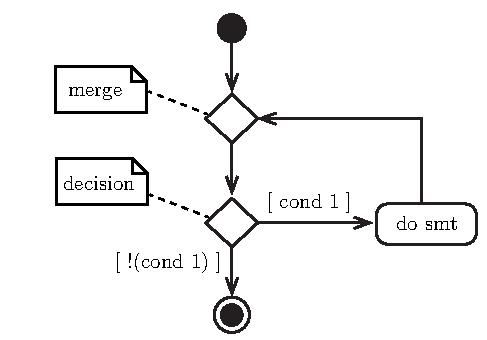
\includegraphics[width=0.50\linewidth]{01_Basics/figures/uml/IterationStatement-00-UML-while.pdf}
% \captionof{figure}{UML \texttt{while} Activity Diagram Representation}
% \label{fig:ch01_Basics_UML_IterationStatement-00-while}
% %~\ref{fig:ch01_Basics_UML_IterationStatement-00-while} 
% %%%%%%%%%%%%%%%%%%%%%%%%%%End figure
% \end{minipage}
% \begin{minipage}{.25\textwidth}
% %%%%%%%%%%%%%%%%%%%%%%%%%%%%%%%%%Begin code
% \begin{lstlisting}[frame=tlrb,numbers=none,mathescape=true,escapechar=\%,columns=flexible]
% some awesome code here
% \end{lstlisting}
% %%%%%%%%%%%%%%%%%%End Code
% \end{minipage}
% \vspace{0.5cm}
% %end minipages


%\begin{enumerate}
%	\item Initialize timer and directions registers
%    \item Specify initial state
%    \item Perform FSM controller
%   \begin{enumerate}
%    	\item Call an output function, which depends on the state
%        \item Delay, which depends on the state
%        \item Call an input function to get the status of the coin sensors
%        \item Change states, which dependes on the state and the input
%    \end{enumerate}
%\end{enumerate}

% \begin{enumerate}
% 	\item Current instruction is finished,
%     \item Eight registers are pushed on the stack,
%     \item LR is set to 0xFFFFFFF9,
%     \item IPSR is set to the interrupt number,
%     \item PC is loaded with the interrupt vector
% \end{enumerate}

% Itemize categoriza poniendo (.) en lugar de números
% \begin{itemize} 
% 	\item I
% 	\item I
% 	\item Y
% 	\item Y
% 	\item Y
% 	\item Y
% 	\item 
% \end{itemize}

% \begin{table}[!h]
% \centering
% \begin{tabular}{|l|l|l|} \hline
% $p$ & bit Field & Interrupt         \\\hline
% $3$ & \bitsRange[31]{29} & Interrupt [$4m+3$]  \\\hline
% $2$ & \bitsRange[23]{21} & Interrupt [$4m+2$]  \\\hline
% $1$ & \bitsRange[15]{13} & Interrupt [$4m+1$]  \\\hline
% $0$ & \bitsRange[7]{5} & Interrupt [$4m$]   \\\hline
% \end{tabular}
% \caption{pasteCaption}
% \label{tab:t_rt_ch04_}
% ~\ref{tab:t_rt_ch04_}
% \end{table}

% Insertar URL
%\url{https://www.osha.gov/Publications/laboratory/OSHAfactsheet-laboratory-safety-noise.pdf}\\

% \newcommand{\bitsRange}[2][50]{\texttt{{#1}-{#2}}}
% \newcommand{\CustomHex}[2][0000]{\texttt{0x{#1}.{#2}}}
% \newcommand{\GPIOPort}[1]{\texttt{GPIO\_PORT{#1}}}
% \newcommand{\GPIOPortR}[2][A]{\texttt{GPIO\_PORT{#1}\_{#2}\_R}}
% \newcommand{\GPIOPortHandler}[1]{\texttt{GPIO\_PORT{#1}\_Handler}}
% \newcommand{\HandlerISR}[1]{\texttt{#1\_Handler}}
% \newcommand{\IRQnr}[1]{\texttt{{#1}}}
% \newcommand{\NVICPRI}[1]{\texttt{NVIC\_PRI{#1}\_R}}
% \newcommand{\NVICEN}[1]{\texttt{NVIC\_EN{#1}\_R}}
% \newcommand{\NVICDIS}[1]{\texttt{NVIC\_DIS{#1}\_R}}
% \newcommand{\Ttimer}[2][A]{\texttt{Timer\_{#2}{#1}}}
% \newcommand{\xNrbit}[1]{$#1$-\texttt{bit}}
% \newcommand{\xNrbits}[1]{$#1$-\texttt{bits}}
% \newcommand{\camouflagegreenCellColor}{\cellcolor[rgb]{0.47, 0.53, 0.42}}
% \newcommand{\lavenderCellColor}{\cellcolor[rgb]{0.9, 0.9, 0.98}}
% \newcommand{\volties}[2][0]{$\si{{#1}\volt}_{#2}$}
% \newcommand{\volti}[1]{$\si{{#1}\volt}$}
% \newcommand{\voltiposi}[1]{$+\si{{#1}\volt}$}
% \newcommand{\voltinega}[1]{$-\si{{#1}\volt}$}